\section{Experimental Results}

% compare things against polling/triggered
% compare things against matchlist length / hashed Portals / multi-PTEs


%We have gathered preliminary performance results using a prototype
%implementation of \pdht running on the Portals reference
%implementation~\cite{portals-code}. Results were gathered on a cluster system
%part of the Advanced Systems Technology Test Bed at Sandia National
%Laboratories.  The cluster contains 36 compute nodes, constructed with dual
%16-core Intel\regtm Haswell\regtm processors and 128 gigabytes of memory. Nodes
%are connected using a Mellanox\othertm FDR 56Gb/s Infiniband\othertm fabric.

Performance results were gathered using a prototype implementation of \pdht
running on a modified version the Portals reference
implementation~\cite{portals-code}. Results were gathered on the Comet cluster
system at the San Diego Supercomputer Center with access provided through the
Extreme Science and Engineering Discovery Environment (XSEDE) program. Comet
contains nodes with several configurations, these experiments were conducted a
portion of the 1944 nodes with Intel\regtm Xeon\regtm E5 processors, comprising
Dell\othertm PowerEdge\othertm C6320 server each with dual 12-core Intel\regtm
Xeon\regtm E5-2680 processors and 128 gigabytes of memory. Nodes are connected
using a Mellanox\othertm FDR 56Gb/s Infiniband\othertm fabric.

\subsection{Experimental Setup}

To measure the effectiveness of implementing PDHT directly on top of Portals,
we constructed an MPI version of PDHT. The MPI version provides a similar
functionality to PDHT and is implemented with separate processes to act as
initiator and target roles to handle insertion, access, and update requests.
The MPI version relies on the same hash function to determine rank and match
bits, but internally uses an efficient hash table on each local
process~\cite{uthash} to store the data elements, keyed with the same 64-bit
value returned by the PDHT hash function. 

%All tests are run using the MPICH 3.2 MPI run-time, configured to use a Portals
%4 channel for all communication operations.

Experiments run with OpenMPI are using version 3.0.0, which has been configured
to use Portals 4 as the message transport layer for all communication
operations. The MPICH MPI tests are run with version 3.2.1 using Portals 4 as
the {\tt ch3} interface. The MVAPICH2 tests are run with version 2.1 and the
runtime is configured to directly use the Infiniband\othertm Verbs interface.

One of the primary challenges in deriving performance results for this work is
that the Portals 4 runtime library was developed as an exploratory framework
for modeling next-generation hardware offload network processing. To this end,
it has not been optimized as extensively as other high-performance network
middleware (e.g. MVAPICH2). Our evaluation of the system focuses on the relative
performance between systems.

%Results from both native PDHT and MPI-based applications that use the reference implementation are skewed by this
%difference in focus. 

% latency
% need to talk about OpenMPI, PDHT, and mvapich

% match list issues
%  - straight bad
%  - multiple PTE
%  - unordered matching
%  - local search

% scaling
%  MPI communication is more expensive than simple PDHT, matching mvapich2
% performance is good, shows that with lower latency performance would be better


\subsection{Communication Operation Costs}

\begin{figure}[ht]
  \center
  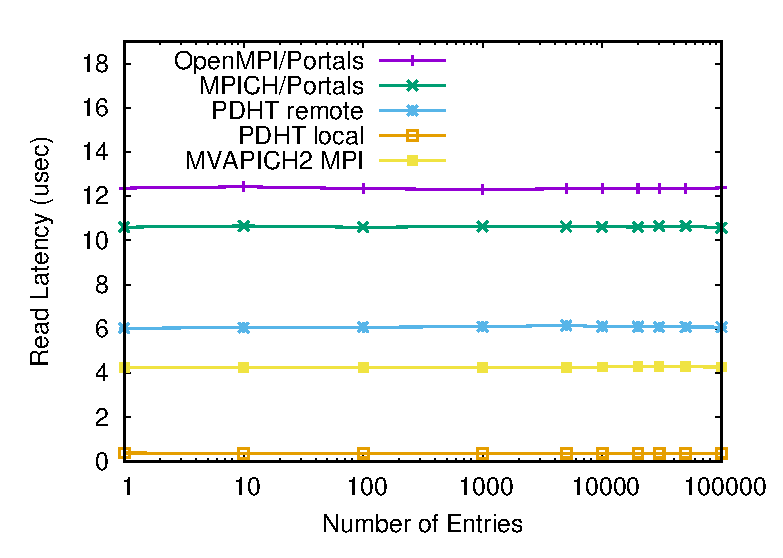
\includegraphics[width=.95\linewidth]{plots/mpilatency}
  \caption{PDHT and MPI Access Latency ($\mu$sec)}
  \label{fig:all-latency}
\end{figure}

\begin{figure}[ht]
  \center
  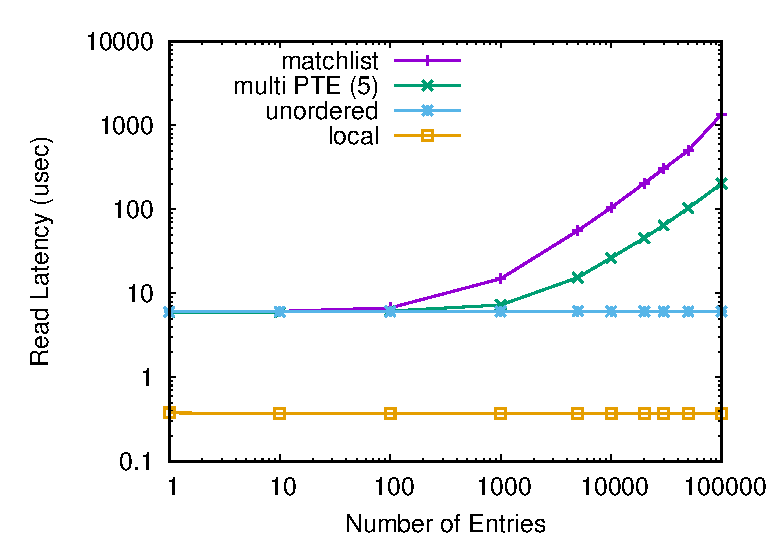
\includegraphics[width=.95\linewidth]{plots/pdhtlatency}
  \caption{PDHT Access Latencies ($\mu$sec)}
  \label{fig:pdht-latency}
\end{figure}


To start with, we evaluate the read latency of our different PDHT
implementations. As can be seen in Figure~\ref{fig:all-latency}, the latency of
the native PDHT implemented directly on Portals is faster than that of the MPI
implementations tested with both MPICH and OpenMPI using Portals communication
channels. This microbenchmark tests the latency with match lists of a varying
number of items. The MPI PDHT implementation tested with the MVAPICH2 system
outperforms all Portals implementations in a raw performance test. We attribute
this to the different design goals of the two systems as mentioned above. Of
particular note are the greatly increasing latencies for the initial native
PDHT implementation. This is caused by the default linked-list searching in the
Portals reference implementation. When using the unordered matching option, the
native PDHT access times are flat over all match list lengths.


Next, we examine the impact of different native PDHT implementation techniques
described in the implementation section. Figure~\ref{fig:pdht-latency} compares
the default version with growing latencies with respect to match list length.
By spreading the key/value entries over multiple Portal table entries (i.e.
multiple match lists), we see that this improves performance, but still causes
latencies to grow as more entries are added. Using the unordered matching
feature in the current version of Portals, we see that PDHT is able to run with
good, flat latencies as the number of local entries increases. Lastly, we see
the impact of searching the local match list rather than performing a full {\tt
  PtlGet()} when fetching entries on the local process rank. This lowers the
access latency by an order of magnitude.

\begin{figure}
    \centering
    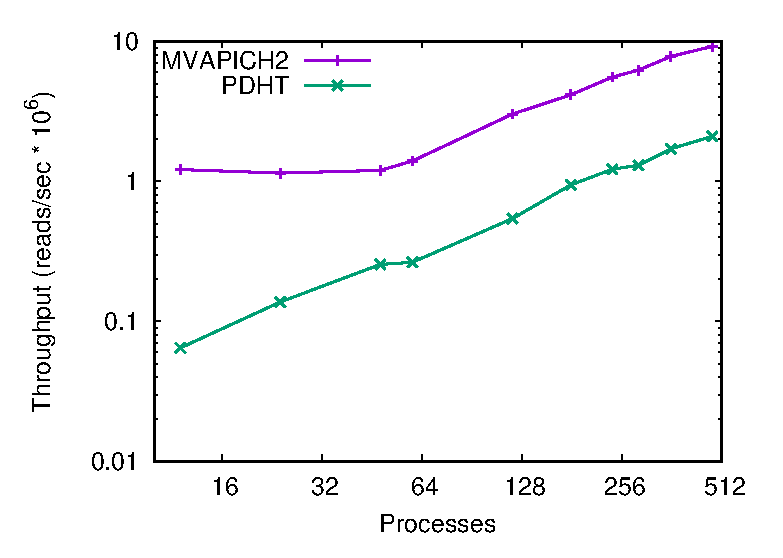
\includegraphics[width=.9\linewidth]{plots/scaling1k}
    %\caption{System throughput for a range of local volume (entries per node).}
    \caption{Aggregate system throughput (1K elements).}
    \label{fig:throughput-small}
\end{figure}

\begin{figure}
    \centering
    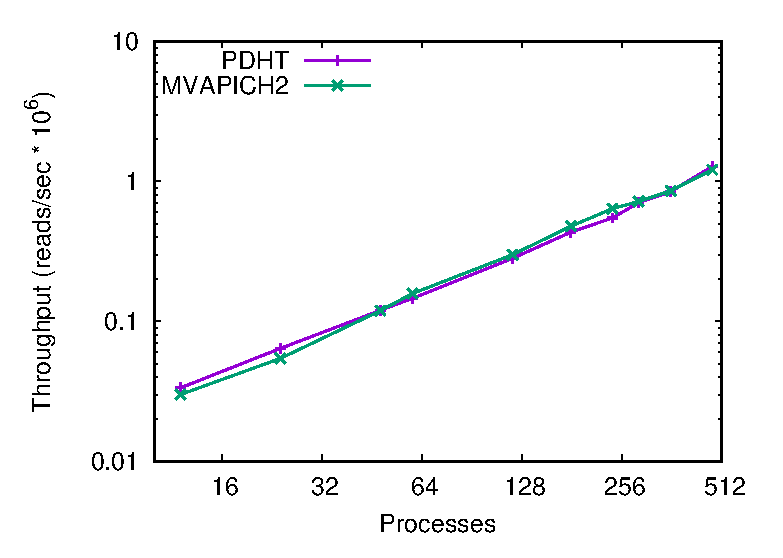
\includegraphics[width=.9\linewidth]{plots/scaling64}
    %\caption{System throughput for a range of local volume (entries per node).}
    \caption{Aggregate system throughput (64K elements).}
    \label{fig:throughput-big}
\end{figure}

As shown in Figure~\ref{fig:throughput-small}, we measure the weak scaling
of \pdht read operations on the key/value store by examining the
overall throughput of the system. Each process owns a fixed number of
hash table elements which are read by a neighboring process. The
system performs as expected under weak scaling, with overall system
throughput increasing with the number of processes involved. We compare
PDHT native performance against MPI using the MVAPICH2 runtime. With smaller
entry sizes, we can see that MVAPICH2 performs better than PDHT. 

This performance gap is largely due to the increased latencies when using a
Portals-based implementation. By increasing the size of a key/value entry to
64KB, we minimize the impact of latency on this benchmark.
Figure~\ref{fig:throughput-big} shows the convergence in overall system
throughput. Portals-based MPI implementations did not scale favorably with
either native or optimized MPI. XXX This is where we should do some 
analysis with round-trip communications in native vs. MPI implementations. It's late.


%To verify this, we measure the performance of retrieving elements from
%the \pdht with respect to the number of elements on each process.
%These results are shown in Figure~\ref{fig:mlen} and provide an
%initial characterization of the lookup cost associated with our \pdht
%implementation.  In contrast with traditional PGAS approaches,
%building a remotely accessible key/value store on top of a mechanism
%intended to support MPI message matching can add new overheads.  In
%particular, the Portals message processing engine must traverse the
%active match list until an ME that matches the given query is located.
%In cases where the element does not exist, the Portals layer must
%reach the end of the list to make this conclusion.  Thus, there is a
%list traversal overhead that is proportional to the number of elements
%visited before finding a match.

It is also useful to explore how the design of the PDHT system can reduce the
number of collisions that occur when compared with  more traditional direct
array-indexed distributed tables. The benchmark code used in another comparison
of UPC, MPI, and SHMEM-based approaches to distributed hash
tables~\cite{maynard:12} was adapted for use with PDHT. This benchmark is
designed to create collision conditions with moderately sized tables. We
compared the OpenSHMEM version of this benchmark against PDHT and found that
with an 80,000 element local table size, the OpenSHMEM implementation had
79,542 collisions for 160,000 insertions. The same set of insertions made with
PDHT resulted in no collisions, due to the indirection provided by the
64-bit match bits as opposed to a direct array index. In practice, we have
not seen collisions in any of the benchmarks described in this section.



% XXX Collisions
%  numbers from SOS vs PDHT benchmark 300K/host

% latency with MPI vs. native
% throughput with MPI vs. native
% matchlist performance
% performance relative OpenSHMEM hash table implementation
% performance of MADNESS reconstruction MPI vs. native
% performance of MADNESS compression MPI vs. native
% performance of MADNESS diff MPI vs. native
% performance of sparse-matrix operation, MPI vs. native




%\subsection{Sparse Matrix Multiplication}
%
%This benchmark application computes the matrix product of two sparse 
%matrices. Matrix sparsity is maintained by decomposing the source
%matrices into tiles containing non-zero and zero elements. Tiles 
%containing non-zero elements are added to the PDHT at the beginning of
%the computation. The matrix multiplication then operates in a SPMD
%fashion with each process requesting the necessary tiles to compute
%the partial product. If either of the operand tiles are not in the
%key/value store, the process continues on until it reaches a tile 
%with non-zero elements. The performance of this benchmark is shown in
%Figures~\ref{fig:4} and \ref{fig:5}.
%
%\begin{figure}[ht]
%  \center
%  \fbox{\rule{2.5in}{0pt}\rule[-2.5in]{0pt}{4ex}}  
%  \caption{Sparse-matrix multiplication weak scaling}
%  \label{fig:4}
%\end{figure}
%
%\begin{figure}[ht]
%  \center
%  \fbox{\rule{2.5in}{0pt}\rule[-2.5in]{0pt}{4ex}}  
%  \caption{Sparse-matrix multiplication strong scaling}
%  \label{fig:5}
%\end{figure}
%


\subsection{MADNESS}

The MADNESS multiresolution numerical computation framework~\cite{thornton09}
has been used to solve a variety of quantum chemistry problems at scale. The
system utilizes wavelet-based functions implemented using 3 to 6 dimensional
spatial representation trees. MADNESS trees represent functions with
coefficients stored in either a scaling basis or a wavelet basis. Certain
operations on the function tree can only be performed in one or the other basis
modes. These spatial decomposition trees are sparse structures, with larger
subtrees corresponding to higher-frequency components of the modeled function.
PDHT can be used to provide a PGLAS system that represents each tree node in
terms of it's spatial coordinates and location (depth) within the tree.

We consider three operations provided by the MADNESS framework. The
first two are conversion operations: {\em compression}, in which scaling
coefficients are converted to the wavelet basis, and {\em reconstruction}, the
complementary operation. The last operation is {\em differentiation}, in which
the derivative of a function tree is computed with respect to a single
dimension. 

\begin{figure}[ht]
  \center
  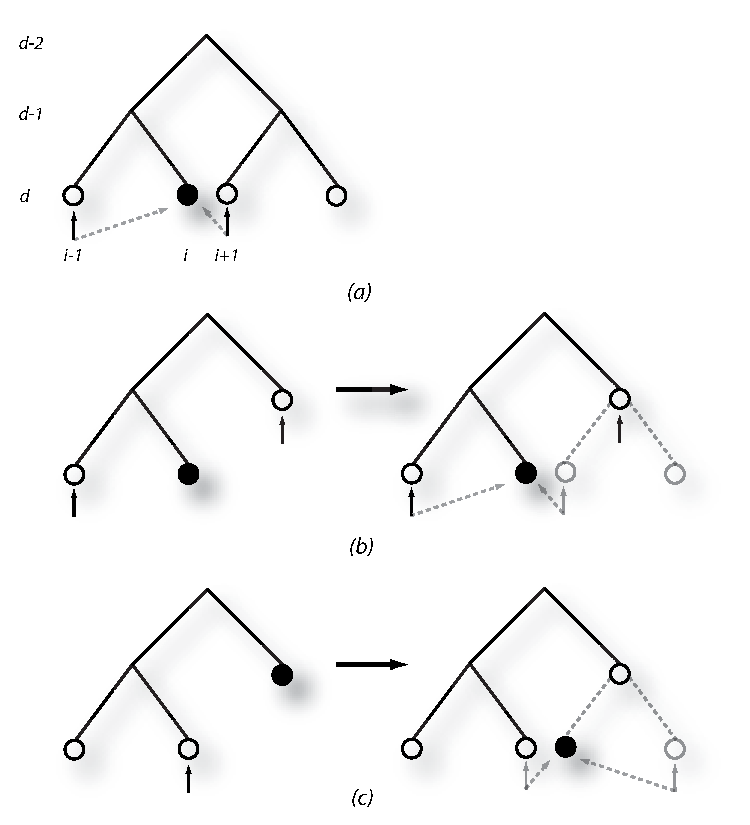
\includegraphics[width=.75\linewidth]{figs/diff}
  \caption{MADNESS differentiation operation}
  \label{fig:diff}
\end{figure}


The differentiation operation is an irregular operation and is easily expressed
using spatial tree coordinates, but is very difficult using traditional
message-passing (due to tree irregularity) and PGAS (due to physical addressing
requirements). As shown in a Fig.~\ref{fig:diff}a with a 1-D function tree,
taking the derivative at node $i$, requires a convolution with coefficients
from nodes $i-1$ and $i+1$ at the same level within the tree. If these nodes
do not exist, the closest ancestor node must be found and expanded to provide
coefficients at the correct level. 


Figures~\ref{fig:mad-compress}--\ref{fig:mad-diff} show the performance of the
Portals-based PDHT implementation relative to the MPI implementation.

\begin{figure}[ht]
  \center
  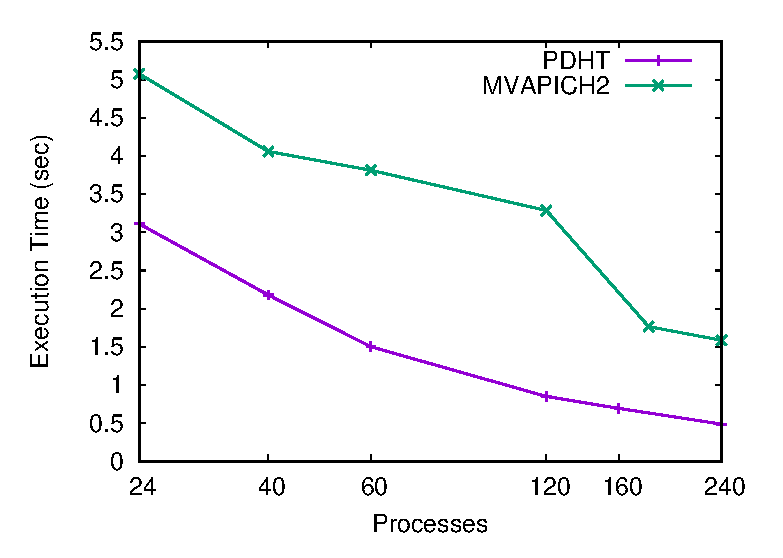
\includegraphics[width=.9\linewidth]{plots/compress}
  \caption{MADNESS compression performance ($\mu$ sec)}
  \label{fig:mad-compress}
\end{figure}

\begin{figure}[ht]
  \center
  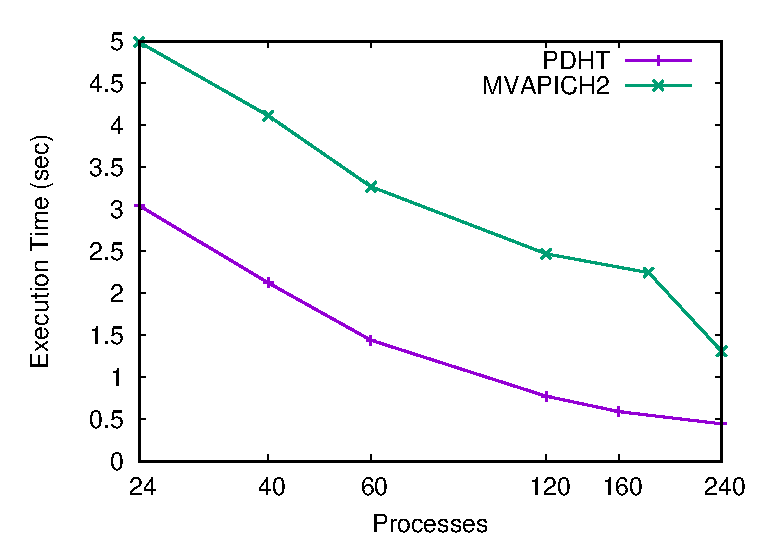
\includegraphics[width=.9\linewidth]{plots/reconstruct}
  \caption{MADNESS reconstruction performance ($\mu$ sec)}
  \label{fig:mad-reconstruct}
\end{figure}


\begin{figure}[ht]
  \center
  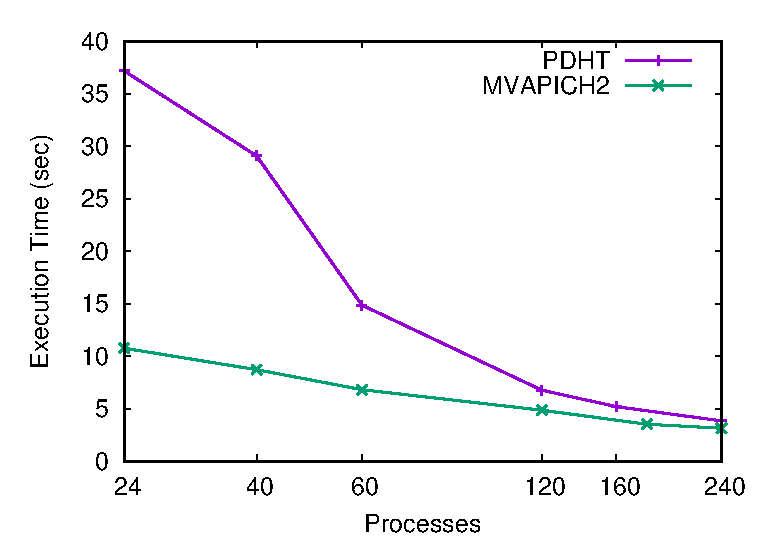
\includegraphics[width=.9\linewidth]{plots/diff}
  \caption{MADNESS differentiation performance ($\mu$ sec)}
  \label{fig:mad-diff}
\end{figure}

\subsection{Meraculous}

The NERSC Meraculous benchmark performs de novo whole genome assembly,
reconstructing genomic sequences from overlapping and erroneous fragments
produced by a high-throughput sequencer. Meraculous constructs a graph of all
overlapping substrings in the input and traverses the graph to discover all
linear subgraphs. These subgraphs correspond to contiguous sequences of
genomic data. Meraculous is written in UPC and uses a hash table
to represent the de Bruijn graph. 

We have adapted the Meraculous benchmark to use PDHT to store the de Bruijn
graph in the place of the UPC hash table. Both structures utilize the same key
structure and creation algorithm. The graph traversal is performed in parallel
by iterating through all local entries in the table and walking both the left
and right ends of the sequence. The results of this experiment are shown in
Figure~\ref{fig:meraculous}. The input file for this experiment was the {\tt
  human-chr14.txt.ufx.bin} data set available as a part of the NERSC benchmark
suite. This input set consists of 96 million sequences, each of which must have
an ME in Portals. At small scale, this consumes a much greater number of
Portals resources than is typically supported. On the other end, adding 
processes reduces Portals resources, but runs out of work quickly.

\begin{figure}[ht]
  \center
  \fbox{\rule{2.5in}{0pt}\rule[-2.5in]{0pt}{4ex}}  
  \caption{Meraculous UPC vs PDHT performance($\mu$ sec)}
  \label{fig:meraculous}
\end{figure}


%%% Local Variables:
%%% mode: latex
%%% TeX-master: "paper"
%%% End:
